% =====================================================================
% Rozdział 2 – Analiza stanu wiedzy (WZÓR, ok. 7–8 stron z rysunkami)
% Styl bezosobowy. Wszystkie fakty pochodzą z kart w praca/materialy/03_streszczenia_artykulow.md.
% Rysunki z artykułów: materialy/rysunki_z_artykulow/ (ścieżki względem folderu praca/).
% Domyślnie włączone: 4 rysunki (Zitová, Oniga, U-Net, Taha) i 2 tabele. Rysunki Hermana i Hana są
% zakomentowane (OPCJA). Jeśli rozdział przekroczy 8 stron: usuń rys. Zitovej (fig:etapy-rejestracji),
% potem tabelę tab:panderm (liczby zostaw w tekście).
% Bez osobnych źródeł (decyzje 26.10): informację wzajemną cytuje się przez zitova2003/correlation-ratio (wariant Mattesa tylko jako metryka SimpleITK, rozdz. 6);
% nazwy GrabCut nie podaje się (,,segmentacja interaktywna z OpenCV''); ViT tylko jako koder PanDerm (yan2025panderm); analizy Blanda--Altmana nie opisuje się.
% =====================================================================

\chapter{Analiza stanu wiedzy}
\label{chap:stan-wiedzy}

W rozdziale omówiono kolejno: obrazowanie zmian skórnych w świetle widzialnym i w podczerwieni, metody rejestracji obrazów wielomodalnych, segmentację obrazów medycznych oraz miary oceny rejestracji i segmentacji. Rozdział zamyka zestawienie prac najbliższych tematowi i wskazanie luki, którą wypełnia niniejsza praca.

% ---------------------------------------------------------------------
\section{Obrazowanie zmian skórnych}
\label{sec:obrazowanie}

Podstawą oceny zmian barwnikowych jest obraz w świetle widzialnym. Dermatoskopia ogranicza odbicie światła od powierzchni skóry i uwidacznia struktury niewidoczne gołym okiem, a komputerowa analiza obrazów dermatoskopowych obejmuje segmentację zmiany, ekstrakcję cech i klasyfikację~\cite{dermoscopy}. Segmentacja jest pierwszym, a zarazem trudnym etapem tej analizy: utrudniają ją zmienność kształtu, rozmiaru i barwy zmian, włosy, naczynia oraz niejednolite warunki akwizycji~\cite{dermoscopy}. Celebi i in.~\cite{dermoscopy} zwracają uwagę, że metody sztucznej inteligencji można stosować także do zwykłych zdjęć wykonywanych z bliska, które dobrze oddają teksturę powierzchni skóry.

Termografia rejestruje promieniowanie podczerwone emitowane przez skórę. Emisyjność skóry wynosi 0,96--0,98, a maksimum jej emisji przypada na zakres 9--12~µm~\cite{infared-thermal-imaging}. Termogram przedstawia wyłącznie rozkład temperatury powierzchni, a wiarygodność pomiaru zależy od standaryzacji badania, w tym od powtarzalnego wyznaczania obszaru zainteresowania -- jego kształt, rozmiar i położenie wpływają na wynik diagnostyczny~\cite{infared-thermal-imaging}.

W termografii statycznej obraz rejestruje się bez stymulacji, a w dynamicznej -- po bodźcu termicznym, chemicznym lub mechanicznym~\cite{magalhaes2019}. Herman i Pirtini Cetingul~\cite{visualization-detection-cancer} chłodzą zmianę wraz z otoczeniem o średnicy 50~mm strumieniem zimnego powietrza przez 1~min, a następnie co 2~s rejestrują powrót temperatury trwający 3--4~min. Ponieważ bez schłodzenia zmiana jest niewidoczna na termogramie, wokół niej przykleja się kwadratowy znacznik, którego narożniki służą do rejestracji zdjęcia z sekwencją obrazów w podczerwieni. Magalhaes i in.~\cite{magalhaes2019} porównali termografię statyczną i dynamiczną dla 46 zmian (16 czerniaków i 30 znamion) zarejestrowanych kamerą o rozdzielczości 320~$\times$~240 pikseli; najlepszy klasyfikator, wykorzystujący cechy statyczne, osiągnął dokładność 84,2\% przy czułości 91,3\%. Obszar analizy wyznaczano tam ręcznie jako okno 40~$\times$~40 pikseli umieszczane przez użytkownika.

% OPCJA (rys. z pracy Hermana – znacznik na skórze i termogram po schłodzeniu): odkomentuj, jeśli zmieści się w limicie 8 stron.
% \begin{figure}[htbp]
%   \centering
%   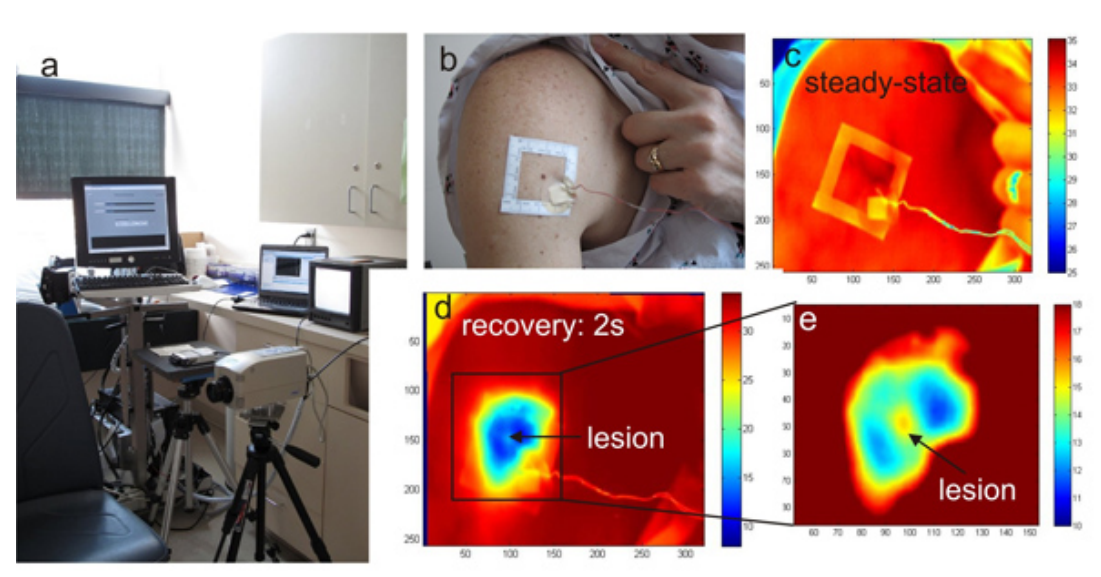
\includegraphics[width=\textwidth]{materialy/rysunki_z_artykulow/R01_herman2011_fig1.png}
%   \caption{Stanowisko do termografii dynamicznej oraz zmiana barwnikowa ze znacznikiem: a)~system obrazowania, b)~zdjęcie skóry z naklejoną ramką, c)~obraz w podczerwieni w temperaturze otoczenia, d)~ten sam obszar po schłodzeniu, e)~powiększenie zmiany. Źródło:~\cite{visualization-detection-cancer}}
%   \label{fig:herman}
% \end{figure}

Obraz widzialny i obraz podczerwony są komplementarne: pierwszy ma bogatą teksturę, lecz zależy od oświetlenia, drugi niesie informację termiczną niezależną od oświetlenia, ale ubogą w szczegóły~\cite{deep-learning}. Łączenie obu modalności wymaga jednak ich wcześniejszej rejestracji, omówionej w kolejnym podrozdziale.

% ---------------------------------------------------------------------
\section{Rejestracja obrazów wielomodalnych}
\label{sec:rejestracja}

\subsection{Modele transformacji i miary podobieństwa}
\label{sec:modele-transformacji}

Rejestracja obrazów to proces nakładania dwóch lub więcej obrazów tej samej sceny wykonanych w różnym czasie, z różnych punktów widzenia lub różnymi sensorami, czyli geometryczne dopasowanie obrazu rejestrowanego do obrazu referencyjnego~\cite{zitova2003}. Zitová i Flusser~\cite{zitova2003} opisują ją czterema etapami: detekcją cech, dopasowaniem cech, estymacją modelu transformacji oraz transformacją i przepróbkowaniem obrazu (rys.~\ref{fig:etapy-rejestracji}). Metody dzieli się na obszarowe (ang.~\textit{area-based}), porównujące bezpośrednio intensywności, oraz oparte na cechach (ang.~\textit{feature-based}). Metody obszarowe wymagają, aby intensywności obu obrazów były identyczne albo przynajmniej statystycznie zależne, natomiast metody oparte na cechach nadają się do rejestracji obrazów z różnych sensorów~\cite{zitova2003}.

\begin{figure}[htbp]
  \centering
  \includegraphics[width=0.6\textwidth]{materialy/rysunki_z_artykulow/R03_zitova2003_fig1.png}
  \caption{Etapy rejestracji obrazów: detekcja cech (u góry), dopasowanie cech (w środku), estymacja modelu transformacji (na dole po lewej) oraz przepróbkowanie obrazu (na dole po prawej). Źródło:~\cite{zitova2003}}
  \label{fig:etapy-rejestracji}
\end{figure}

Wybór modelu transformacji określa, jakie zniekształcenia mogą zostać skompensowane. Model podobieństwa (obrót, przesunięcie, jednolita skala) wyznaczają dwa punkty kontrolne, model afiniczny -- trzy niewspółliniowe punkty; zachowuje on proste i równoległość. Przekształcenie perspektywiczne (homografia) dokładnie opisuje płaską scenę fotografowaną kamerą, której oś optyczna nie jest prostopadła do sceny, i wymaga czterech punktów kontrolnych~\cite{zitova2003}. W pracy~\cite{gonzalezperez2021} homografia, mimo największej liczby stopni swobody, najsłabiej przenosiła się na obrazy wykonane w innej odległości niż obrazy, na których ją wyznaczono. Oniga i in.~\cite{oniga2026} uzasadniają z kolei wybór homografii tym, że niewielki fragment skóry ze sztywnym znacznikiem jest lokalnie quasi-płaski.

W metodach obszarowych transformację wyznacza się przez optymalizację miary podobieństwa. Evangelidis i Psarakis~\cite{evangelidis2008} zaproponowali kryterium rozszerzonego współczynnika korelacji (ang.~\textit{enhanced correlation coefficient}, ECC), które -- dzięki odjęciu średniej i normalizacji wektorów intensywności -- jest niezmiennicze względem zmian jasności i kontrastu. Kryterium jest nieliniowe względem parametrów, dlatego autorzy zaproponowali iteracyjne schematy optymalizacji z rozwiązaniem w postaci zamkniętej w każdej iteracji; w eksperymentach symulacyjnych osiągały one mniejszy błąd i częstszą zbieżność niż odpowiadające im warianty algorytmu Lucasa--Kanade~\cite{evangelidis2008}. Jak wszystkie metody gradientowe, ECC wymaga jednak dobrego punktu startowego i ma trudności w obszarach jednorodnych oraz przy dużych przesunięciach~\cite{evangelidis2008}. W rejestracji wielomodalnej stosuje się miary statystyczne, przede wszystkim informację wzajemną~\cite{zitova2003}, która nie zakłada postaci zależności między intensywnościami; Roche i in.~\cite{correlation-ratio} pokazali jednak na przykładzie syntetycznym, że może ona mieć wiele równoważnych maksimów.

W niniejszej pracy miarę podobieństwa oblicza się nie na surowych obrazach, lecz na maskach znacznika wyodrębnionych w obu modalnościach, co sprowadza problem wielomodalny do jednomodalnego i umożliwia zastosowanie kryterium ECC.

\subsection{Rejestracja obrazów widzialnych i termowizyjnych}
\label{sec:rgb-ir}

Rejestrację obrazów widzialnych i termowizyjnych utrudnia odmienny mechanizm ich powstawania: jasność w podczerwieni zależy od temperatury i emisyjności obiektów, a w świetle widzialnym -- od światła odbitego, więc intensywności nie są bezpośrednio powiązane~\cite{visible-and-infared}. Han i in.~\cite{visible-and-infared} wykazali, że punkty charakterystyczne SURF i Harrisa wykrywane w obu modalnościach w dużej mierze się nie pokrywają. Zaproponowana przez nich metoda wykorzystuje proste wyprowadzone z krawędzi obiektów, przez co wymaga struktur typowych dla otoczenia zbudowanego przez człowieka i nie przenosi się na obrazy skóry.

% OPCJA (rys. z pracy Hana – punkty SURF/Harris): odkomentuj, jeśli zmieści się w limicie 8 stron.
% \begin{figure}[htbp]
%   \centering
%   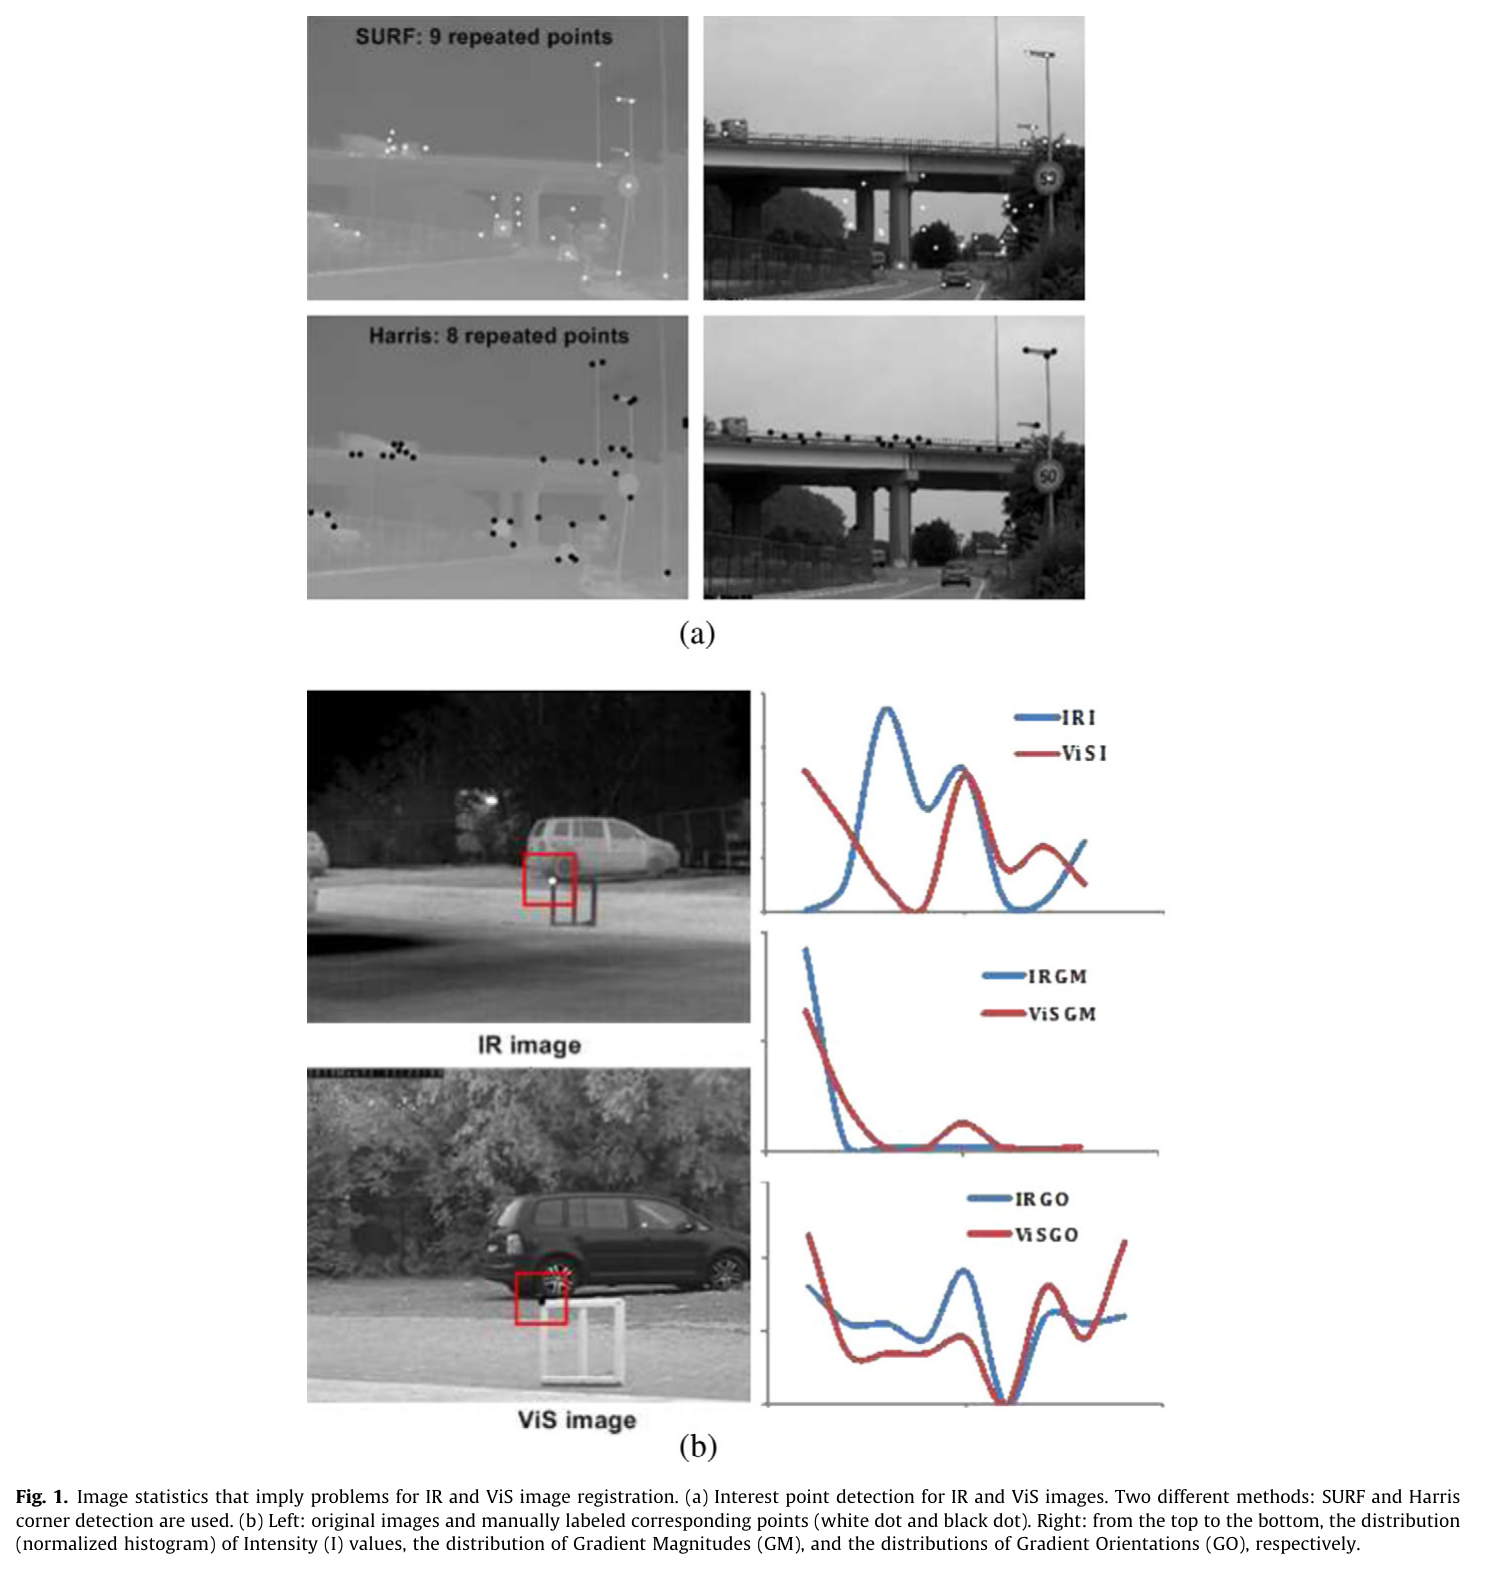
\includegraphics[width=0.6\textwidth]{materialy/rysunki_z_artykulow/R08_han2013_fig1.png}
%   \caption{Problemy rejestracji obrazów podczerwonych i widzialnych: a)~punkty charakterystyczne SURF i Harrisa wykryte w obu modalnościach, b)~rozkłady intensywności i gradientów w odpowiadających sobie fragmentach. Źródło:~\cite{visible-and-infared}}
%   \label{fig:han}
% \end{figure}

W zastosowaniach medycznych korespondencję zapewnia się zwykle obiektem widocznym w obu modalnościach. González-Pérez i in.~\cite{gonzalezperez2021} porównali cztery metody rejestracji obrazów stopy w systemie z kamerami połączonymi na sztywno; punkty kalibracyjne dawała szachownica umieszczona przed schłodzoną płytą aluminiową, kontrastującą termicznie z otoczeniem. Metoda afiniczna optymalizowana na binarnych maskach stóp uzyskała w płaszczyźnie ostrości kamer (800~mm) współczynnik Dice'a 0,982, przy czym na surowych obrazach różnych widm optymalizacja ta nie zbiegała poprawnie~\cite{gonzalezperez2021}. Maurya i in.~\cite{non-contact-breathing-monitoring} wyznaczają punkty kontrolne na ramie kalibracyjnej wyciętej z materiału słabo przewodzącego ciepło, a transformację doprecyzowują cechami opartymi na zgodności fazy, uzyskując średni błąd rejestracji 1,817 piksela dla 50 par obrazów. Obszar zainteresowania wyznaczają i śledzą w obrazie RGB, a następnie przenoszą go na obraz termowizyjny, ubogi w teksturę~\cite{non-contact-breathing-monitoring}.

Najbliższe tematowi niniejszej pracy jest rozwiązanie Onigi i in.~\cite{oniga2026}, którzy rejestrują obrazy zmian skórnych w świetle widzialnym, bliskiej podczerwieni i termowizji z użyciem kwadratowego znacznika umieszczonego na skórze wokół zmiany (rys.~\ref{fig:oniga}). Znacznik lokalizuje detektor YOLOv8n, a homografię wyznacza się z punktów kluczowych przewidywanych przez sieć neuronową. Autorzy zauważają, że w obrazie termowizyjnym znacznik bywa słabiej widoczny i ma zaokrąglone narożniki, a zmiana skórna często nie jest widoczna. Wyniki oceniano wyłącznie miarami podobieństwa obrazów (SSIM, MI, NMI), bez miar geometrycznych~\cite{oniga2026}.

\begin{figure}[htbp]
  \centering
  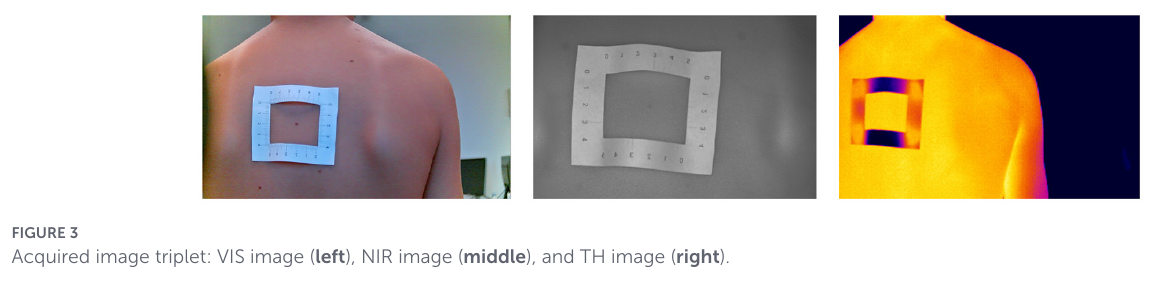
\includegraphics[width=0.8\textwidth]{materialy/rysunki_z_artykulow/R07_oniga2026_fig3.png}
  \caption{Kwadratowy znacznik referencyjny na skórze w obrazie widzialnym (po lewej), w bliskiej podczerwieni (w środku) i w obrazie termowizyjnym (po prawej). Źródło:~\cite{oniga2026}}
  \label{fig:oniga}
\end{figure}

\subsection{Metody oparte na uczeniu głębokim}
\label{sec:rejestracja-dl}

Przegląd Chena i in.~\cite{deep-learning-in-registration}, obejmujący 77 prac, dzieli metody głębokiej rejestracji obrazów medycznych na trzy grupy: sieci pełniące rolę miary podobieństwa, sieci bezpośrednio wyznaczające parametry transformacji (w wariantach nadzorowanym, słabo nadzorowanym i nienadzorowanym) oraz pozostałe zastosowania. Przykładem podejścia słabo nadzorowanego jest praca Hu i in.~\cite{neural-networks}, w której sieć konwolucyjna przewiduje pole przemieszczeń między obrazami MR i TRUS prostaty; etykiety anatomiczne są potrzebne wyłącznie podczas uczenia, a w fazie wnioskowania wystarcza para obrazów. Autorzy uzyskali medianę błędu w punktach docelowych 3,6~mm na 108 parach obrazów, podczas gdy klasyczna rejestracja oparta na miarach intensywności zawiodła na tych danych~\cite{neural-networks}. Metody głębokie wymagają jednak licznych danych uczących, a publicznie dostępnych zbiorów wielomodalnych jest niewiele~\cite{deep-learning-in-registration}. Dla pary telefon--kamera termowizyjna takich danych nie ma, dlatego w niniejszej pracy zastosowano rejestrację klasyczną opartą na znaczniku.

\subsection{Fuzja i wizualizacja nałożenia}
\label{sec:fuzja}

Zhang i Demiris~\cite{deep-learning} wyróżniają fuzję obrazów widzialnych i podczerwonych na poziomie pikseli, cech i decyzji; w literaturze termin ten odnosi się zwykle do poziomu pikseli, na którym powstaje jeden obraz wynikowy. Fuzja pikselowa wymaga dokładnej rejestracji, a autorzy uznają wyrównanie obrazów widzialnych i podczerwonych za problem otwarty, wskazując wspólne uczenie rejestracji i fuzji jako kierunek badań~\cite{deep-learning}. W niniejszej pracy nałożenie obrazów pełni funkcję wizualizacji wyniku rejestracji, a wspólna analiza odbywa się przez przeniesienie obszaru zainteresowania, podobnie jak w~\cite{non-contact-breathing-monitoring}.

% ---------------------------------------------------------------------
\section{Segmentacja obrazów medycznych}
\label{sec:segmentacja}

\subsection{Metody klasyczne}
\label{sec:segmentacja-klasyczna}

Przed upowszechnieniem uczenia głębokiego segmentację zmian skórnych realizowano m.in. progowaniem adaptacyjnym, konturami aktywnymi, rozrostem obszaru i klasteryzacją (za:~\cite{mirikharaji2023}). Metody te opierają się na cechach projektowanych ręcznie, co ogranicza ich skuteczność na dużych i zróżnicowanych zbiorach danych~\cite{mirikharaji2023}. W niniejszej pracy metody klasyczne wykorzystano do detekcji znacznika referencyjnego, który ma znany kształt i wyraźnie kontrastuje ze skórą.

\subsection{Sieć U-Net i architektury koder--dekoder}
\label{sec:unet}

Ronneberger i in.~\cite{ronneberger2015} zaproponowali sieć U-Net do segmentacji obrazów biomedycznych przy bardzo małej liczbie oznaczonych obrazów. Ścieżka kurcząca (koder) gromadzi kontekst, symetryczna ścieżka rozszerzająca (dekoder) zapewnia dokładną lokalizację, a połączenia skrótowe przekazują cechy wysokiej rozdzielczości z kodera do dekodera (rys.~\ref{fig:unet}). Kluczowym elementem uczenia była intensywna augmentacja, zwłaszcza losowe deformacje sprężyste; sieć uczona na 30 obrazach z mikroskopii elektronowej zajęła pierwsze miejsce w rankingu wyzwania ISBI według błędu deformacji~\cite{ronneberger2015}. Według przeglądu~\cite{mirikharaji2023}, obejmującego 177 prac o segmentacji zmian skórnych, połączenia skrótowe stosuje 112 z nich, a najczęstszymi funkcjami straty są entropia krzyżowa i strata Dice.

\begin{figure}[htbp]
  \centering
  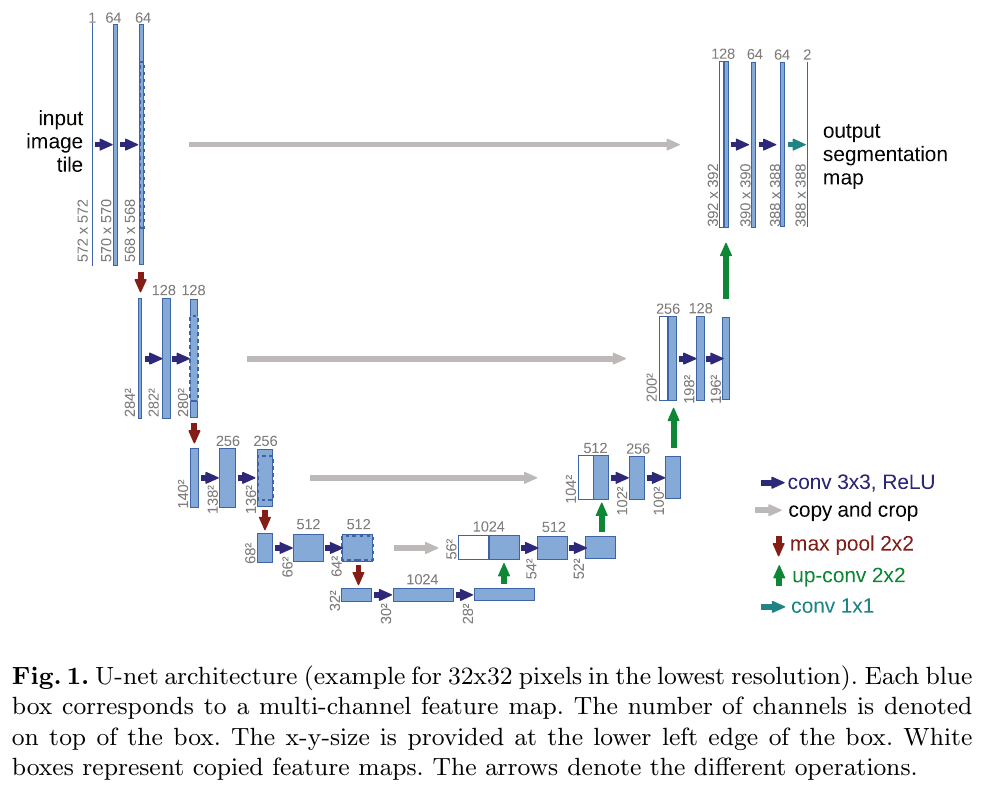
\includegraphics[width=0.6\textwidth]{materialy/rysunki_z_artykulow/R13_ronneberger2015_fig1.png}
  \caption{Architektura sieci U-Net. Prostokąty oznaczają mapy cech (nad nimi liczba kanałów), strzałki -- operacje. Źródło:~\cite{ronneberger2015}}
  \label{fig:unet}
\end{figure}

Dekoder UperNet~\cite{xiao2018upernet} łączy piramidę cech (ang.~\textit{Feature Pyramid Network}, FPN) z modułem łączenia piramidalnego (ang.~\textit{Pyramid Pooling Module}, PPM) dołączonym do najgłębszej warstwy kodera. Moduł PPM wnosi kontekst globalny, a fuzja map cech ze wszystkich poziomów piramidy poprawia wynik segmentacji; w oryginalnej pracy na zbiorze ADE20K konfiguracja FPN~+~PPM z fuzją osiągnęła mIoU 41,22\%~\cite{xiao2018upernet}.

\subsection{Modele bazowe w dermatologii i zbiory danych}
\label{sec:modele-bazowe}

Model bazowy (ang.~\textit{foundation model}) to duża sieć wstępnie uczona samonadzorowanie na dużym, zróżnicowanym zbiorze danych, którą można douczyć do konkretnego zadania przy niewielkiej liczbie etykiet~\cite{yan2025panderm}. PanDerm~\cite{yan2025panderm} to model bazowy dla dermatologii z koderem typu ViT-Large, uczony na 2~149~706 obrazach z 11 źródeł w czterech modalnościach: fotografii całego ciała, dermatopatologii, zdjęciach klinicznych (460~328 obrazów) i obrazach dermatoskopowych. W zadaniu segmentacji, z dekoderem UperNet, model uzyskał Dice 0,910 na zbiorze ISIC 2018 i 0,949 na HAM10000, przewyższając modele porównawcze (tab.~\ref{tab:panderm}); przy 5\% danych uczących dorównywał najlepszemu z pozostałych modeli uczonych na pełnym zbiorze~\cite{yan2025panderm}. Segmentację oceniono jednak wyłącznie na obrazach dermatoskopowych.

\begin{table}[htbp]
  \centering
  \caption{Wyniki segmentacji zmian skórnych modelu PanDerm i modeli porównawczych (DSC -- współczynnik Dice'a, JAC -- indeks Jaccarda). Opracowanie własne na podstawie~\cite{yan2025panderm}}
  \label{tab:panderm}
  \begin{tabular}{lcccc}
    \toprule
    Model & \multicolumn{2}{c}{ISIC 2018} & \multicolumn{2}{c}{HAM10000} \\
     & DSC & JAC & DSC & JAC \\
    \midrule
    SL-ImageNet & 0,876 & 0,807 & 0,927 & 0,875 \\
    autoSMIM    & 0,848 & 0,769 & 0,920 & 0,865 \\
    BATFormer   & 0,884 & 0,815 & 0,937 & 0,891 \\
    PanDerm     & \textbf{0,910} & \textbf{0,846} & \textbf{0,949} & \textbf{0,910} \\
    \bottomrule
  \end{tabular}
\end{table}

Najczęściej wykorzystywanymi zbiorami do segmentacji zmian skórnych są zbiory wyzwań ISIC, użyte w 168 ze 177 prac objętych przeglądem~\cite{mirikharaji2023}. Zbiór zadania segmentacji ISIC 2018 obejmuje 3694 obrazy dermatoskopowe z oficjalnym podziałem na 2594 obrazy uczące, 100 walidacyjnych i 1000 testowych~\cite{codella2019,mirikharaji2023}. Zbiór HAM10000~\cite{tschandl2018} zawiera 10~015 obrazów dermatoskopowych z dwóch ośrodków, zebranych w ciągu 20 lat i przypisanych do siedmiu klas diagnostycznych. W wyzwaniu ISIC 2018 wprowadzono progowany indeks Jaccarda, w którym wynik dla obrazu poniżej 0,65 zastępuje się zerem, traktując segmentację jako porażkę; próg wyznaczono na podstawie zgodności trzech ekspertów, których średni indeks Jaccarda wynosił 0,786~\cite{codella2019}. Problem segmentacji pozostaje otwarty -- najlepsze zgłoszenie uzyskało progowany indeks Jaccarda 0,802, a mimo średnich wartości indeksu Jaccarda powyżej 0,8 większość metod zawodziła na ponad 10\% obrazów, najczęściej w przypadku rogowacenia łojotokowego~\cite{codella2019}. Jednocześnie liczba zdjęć klinicznych z maskami segmentacji od lat pozostaje niewielka w porównaniu z obrazami dermatoskopowymi~\cite{mirikharaji2023}, dlatego modele uczone na dermoskopii stosowane do zdjęć z telefonu pracują w warunkach przesunięcia dziedziny (ang.~\textit{domain shift}).

\subsection{Segmentacja obrazów termowizyjnych}
\label{sec:segmentacja-termo}

Ponieważ znamię bez schłodzenia skóry nie jest widoczne na termogramie, w pracach dotyczących termografii zmian skórnych obrys wyznacza się na obrazie widzialnym i przenosi na obraz w podczerwieni~\cite{visualization-detection-cancer} albo obszar analizy ustawia się ręcznie~\cite{magalhaes2019}. W termowizji można natomiast wyznaczyć obiekt referencyjny o odmiennych własnościach termicznych -- znacznik~\cite{oniga2026}. Z tego względu w niniejszej pracy model segmentacji dedykowany termowizji wyznacza maskę znacznika, a nie znamienia.

% ---------------------------------------------------------------------
\section{Miary oceny rejestracji i segmentacji}
\label{sec:miary}

Fitzpatrick i in.~\cite{fitzpatrick1998} rozróżniają trzy rodzaje błędów rejestracji opartej na punktach: błąd lokalizacji znacznika (ang.~\textit{fiducial localization error}, FLE), błąd dopasowania znaczników po rejestracji (ang.~\textit{fiducial registration error}, FRE) oraz błąd w punkcie docelowym (ang.~\textit{target registration error}, TRE), czyli odległość między odpowiadającymi sobie punktami po rejestracji. Autorzy wykazali, że FRE nie zależy od konfiguracji znaczników i jest zawodnym wskaźnikiem dokładności, natomiast TRE rośnie wraz z odległością celu od środka konfiguracji~\cite{fitzpatrick1998}. Dokładność rejestracji należy więc oceniać na punktach, które nie uczestniczyły w wyznaczaniu transformacji; zdaniem Zitovej i Flussera~\cite{zitova2003} bez oceny ilościowej żadna metoda rejestracji nie może zostać przyjęta do praktycznego zastosowania.

Taha i Hanbury~\cite{taha2015} zestawili 20 miar oceny segmentacji w sześciu kategoriach, m.in. miary pokrycia, objętościowe i odległościowe. Współczynnik Dice'a i indeks Jaccarda są ze sobą powiązane monotonicznie, dlatego dają ten sam ranking segmentacji. Miary pokrycia nie wykrywają błędów kształtu brzegu (rys.~\ref{fig:taha}) i nie są zalecane dla małych obiektów, a odległość Hausdorffa jest wrażliwa na punkty odstające, dlatego zastępuje się ją kwantylem odległości~\cite{taha2015}. Zgodnie z zaleceniami Metrics Reloaded~\cite{maierhein2024}, opracowanymi w procesie delfickim przez międzynarodowe konsorcjum ekspertów, w segmentacji semantycznej miarę pokrycia (DSC lub IoU) uzupełnia się miarą brzegową, np. 95.~percentylem odległości Hausdorffa (HD95) lub średnią symetryczną odległością powierzchni (ASSD). Te same zalecenia wskazują, że miary należy liczyć osobno dla każdego obrazu i agregować z uwzględnieniem hierarchii danych~\cite{maierhein2024}. Podobne podejście -- ocenę rejestracji przez zgodność masek po przeniesieniu -- zastosowano w pracy~\cite{gonzalezperez2021}.

\begin{figure}[htbp]
  \centering
  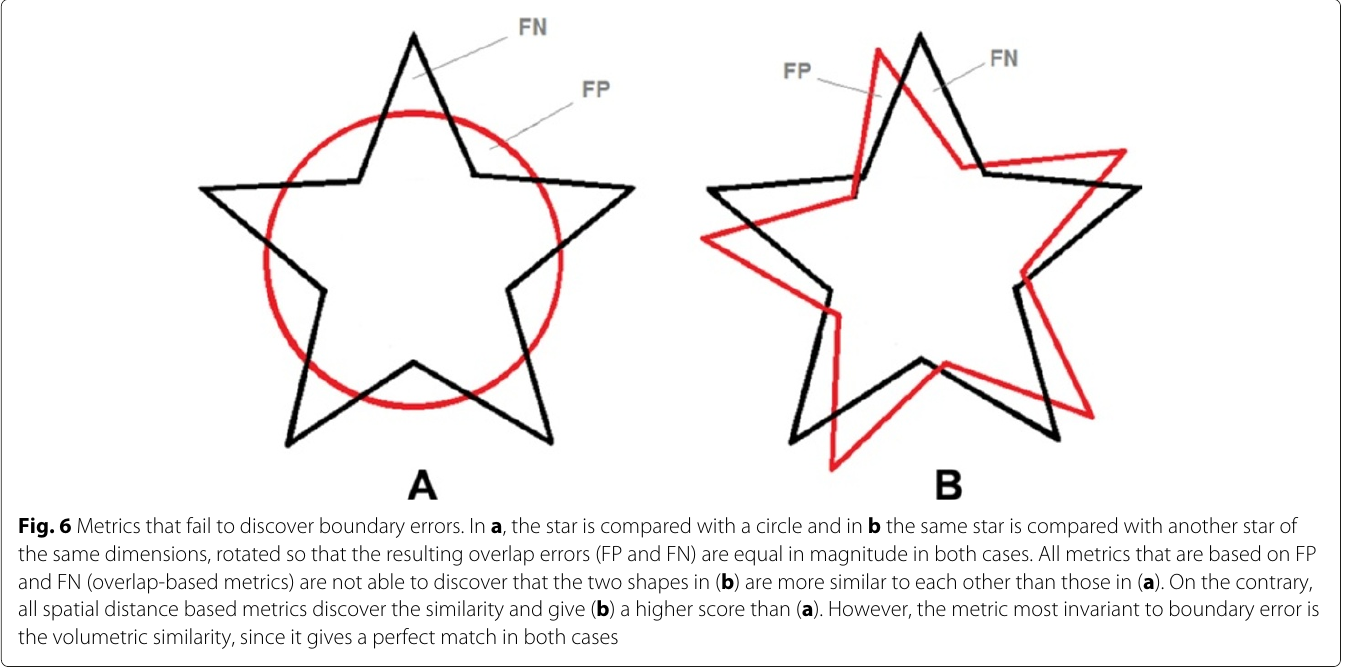
\includegraphics[width=0.65\textwidth]{materialy/rysunki_z_artykulow/R18_taha2015_fig6.png}
  \caption{Przykład, w którym miary pokrycia nie wykrywają błędu brzegu: w obu przypadkach liczby pikseli fałszywie dodatnich i fałszywie ujemnych są równe, mimo różnego podobieństwa kształtów. Źródło:~\cite{taha2015}}
  \label{fig:taha}
\end{figure}

W niniejszej pracy dokładność rejestracji oceniano błędem TRE wyznaczanym na narożnikach znacznika oznaczonych ręcznie, które nie uczestniczą w wyznaczaniu transformacji, a zgodność masek -- współczynnikiem Dice'a uzupełnionym miarami HD95 i ASSD wyrażonymi w milimetrach.

% ---------------------------------------------------------------------
\section{Podsumowanie i luka badawcza}
\label{sec:luka}

Zestawienie prac rejestrujących obraz widzialny z termowizyjnym przedstawiono w tabeli~\ref{tab:prace-rgb-ir}. We wszystkich rozwiązaniach przeznaczonych dla medycyny korespondencję między modalnościami zapewnia obiekt referencyjny, a obszar zainteresowania wyznacza się w obrazie widzialnym. Prace różnią się jednak sposobem oceny: stosowano błąd w pikselach, zgodność masek albo miary podobieństwa obrazów, a w żadnej z nich nie weryfikowano zgodności przeniesionego obszaru niezależnym modelem segmentacji drugiej modalności.

\begin{table}[htbp]
  \centering
  \caption{Prace rejestrujące obraz widzialny z obrazem termowizyjnym. Opracowanie własne na podstawie~\cite{visualization-detection-cancer,visible-and-infared,non-contact-breathing-monitoring,gonzalezperez2021,oniga2026}}
  \label{tab:prace-rgb-ir}
  \small
  \begin{tabularx}{\textwidth}{>{\raggedright\arraybackslash}p{2.4cm} >{\raggedright\arraybackslash}X >{\raggedright\arraybackslash}X >{\raggedright\arraybackslash}X}
    \toprule
    Praca & Zastosowanie & Źródło korespondencji & Ocena rejestracji \\
    \midrule
    Herman i Pirtini Cetingul~\cite{visualization-detection-cancer} & termografia dynamiczna zmian barwnikowych & narożniki kwadratowego znacznika na skórze & brak miar ilościowych \\
    Han i in.~\cite{visible-and-infared} & sceny zurbanizowane & proste z krawędzi obiektów, punkty Harrisa & błąd w pikselach \\
    Maurya i in.~\cite{non-contact-breathing-monitoring} & pomiar częstości oddechu & rama kalibracyjna, cechy zgodności fazy & TRE 1,817 piksela (50 par) \\
    González-Pérez i in.~\cite{gonzalezperez2021} & monitorowanie stopy cukrzycowej & szachownica z płytą aluminiową, maski stóp & Dice i Jaccard masek \\
    Oniga i in.~\cite{oniga2026} & zmiany skórne (VIS, NIR, TH) & kwadratowy znacznik, punkty z sieci neuronowej & SSIM, MI, NMI \\
    Niniejsza praca & zmiany skórne & kształt znacznika $\Pi$ (maski w obu modalnościach) & TRE w mm, zgodność masek z modelu segmentacji termowizji \\
    \bottomrule
  \end{tabularx}
\end{table}

Z przeglądu wynikają trzy wnioski dla projektu systemu. Po pierwsze, ze względu na brak wspólnych cech naturalnych i niewidoczność znamienia na termogramie korespondencję należy oprzeć na znaczniku widocznym w obu modalnościach. Po drugie, brak dużego zbioru par telefon--termogram przemawia za klasyczną rejestracją na maskach znacznika, a w segmentacji -- za douczaniem modelu bazowego i niewielkimi sieciami typu U-Net. Po trzecie, ocena powinna łączyć błąd w punktach docelowych z miarami pokrycia i miarami brzegowymi. W przeanalizowanej literaturze nie znaleziono systemu, który rejestruje zdjęcie z telefonu z termogramem na podstawie znacznika o znanym kształcie i weryfikuje zgodność przeniesionego obszaru modelem segmentacji dedykowanym drugiej modalności, bez potrzeby ręcznych adnotacji. Lukę tę wypełnia niniejsza praca.
